\documentclass{standalone}
\usepackage{tikz}
\usetikzlibrary{patterns, positioning}

\begin{document}
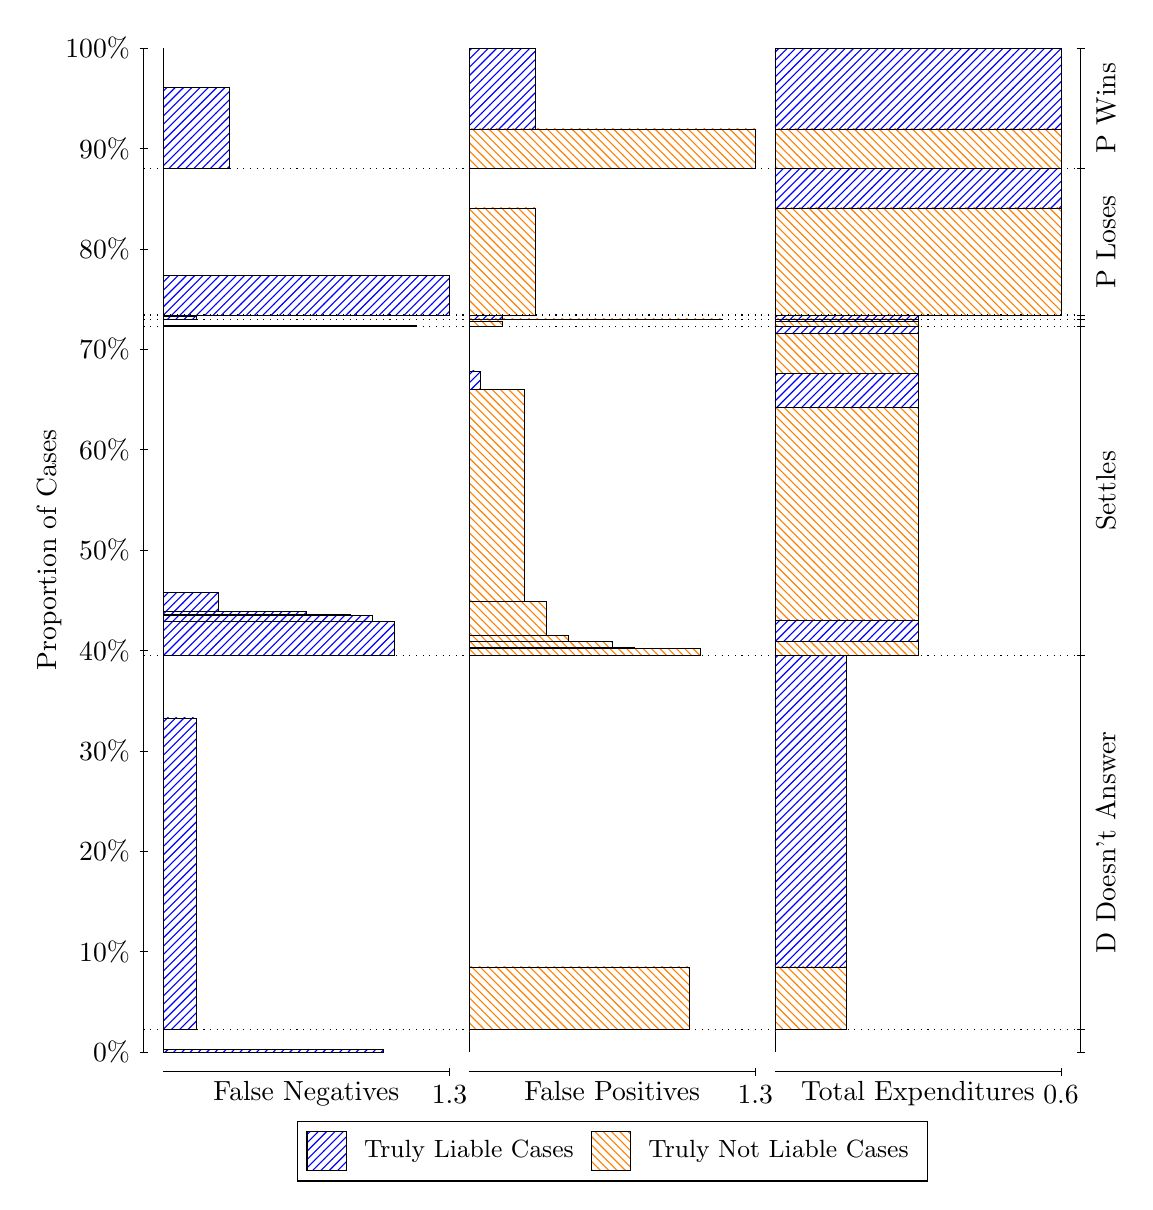
\begin{tikzpicture}
\draw[black, very thin] (1.5,1.75) -- (1.5,14.5);
\node[rotate=90, anchor=center] at (0.3, 8.125) {Proportion of Cases};
\draw[black, very thin] (1.45,1.75) -- (1.55,1.75);
\node[anchor=east] at (1.45, 1.75) {0\%};
\draw[black, very thin] (1.45,3.025) -- (1.55,3.025);
\node[anchor=east] at (1.45, 3.025) {10\%};
\draw[black, very thin] (1.45,4.3) -- (1.55,4.3);
\node[anchor=east] at (1.45, 4.3) {20\%};
\draw[black, very thin] (1.45,5.575) -- (1.55,5.575);
\node[anchor=east] at (1.45, 5.575) {30\%};
\draw[black, very thin] (1.45,6.85) -- (1.55,6.85);
\node[anchor=east] at (1.45, 6.85) {40\%};
\draw[black, very thin] (1.45,8.125) -- (1.55,8.125);
\node[anchor=east] at (1.45, 8.125) {50\%};
\draw[black, very thin] (1.45,9.4) -- (1.55,9.4);
\node[anchor=east] at (1.45, 9.4) {60\%};
\draw[black, very thin] (1.45,10.675) -- (1.55,10.675);
\node[anchor=east] at (1.45, 10.675) {70\%};
\draw[black, very thin] (1.45,11.95) -- (1.55,11.95);
\node[anchor=east] at (1.45, 11.95) {80\%};
\draw[black, very thin] (1.45,13.225) -- (1.55,13.225);
\node[anchor=east] at (1.45, 13.225) {90\%};
\draw[black, very thin] (1.45,14.5) -- (1.55,14.5);
\node[anchor=east] at (1.45, 14.5) {100\%};

\draw[black, very thin] (13.4,1.75) -- (13.4,14.5);
\draw[black, very thin] (13.35,1.75) -- (13.45,1.75);
\node[anchor=west] at (13.35, 1.75) {};
\draw[black, very thin] (13.35,2.0384) -- (13.45,2.0384);
\node[anchor=west] at (13.35, 2.0384) {};
\draw[black, very thin] (13.35,6.7843) -- (13.45,6.7843);
\node[anchor=west] at (13.35, 6.7843) {};
\draw[black, very thin] (13.35,10.967) -- (13.45,10.967);
\node[anchor=west] at (13.35, 10.967) {};
\draw[black, very thin] (13.35,11.049) -- (13.45,11.049);
\node[anchor=west] at (13.35, 11.049) {};
\draw[black, very thin] (13.35,11.109) -- (13.45,11.109);
\node[anchor=west] at (13.35, 11.109) {};
\draw[black, very thin] (13.35,12.972) -- (13.45,12.972);
\node[anchor=west] at (13.35, 12.972) {};
\draw[black, very thin] (13.35,14.5) -- (13.45,14.5);
\node[anchor=west] at (13.35, 14.5) {};

\draw[black, very thin, pattern color=blue, pattern=north east lines] (1.75,1.75) rectangle (4.5449,1.7803);
\draw[black, very thin, pattern color=orange, pattern=north west lines] (1.75,1.7803) rectangle (1.75,2.0384);
\draw[black, very thin, pattern color=blue, pattern=north east lines] (1.75,2.0384) rectangle (2.1692,5.9922);
\draw[black, very thin, pattern color=orange, pattern=north west lines] (1.75,5.9922) rectangle (1.75,6.7843);
\draw[black, very thin, pattern color=blue, pattern=north east lines] (1.75,6.7843) rectangle (4.6846,7.2184);
\draw[black, very thin, pattern color=blue, pattern=north east lines] (1.75,7.2184) rectangle (4.4051,7.2913);
\draw[black, very thin, pattern color=blue, pattern=north east lines] (1.75,7.2913) rectangle (4.1256,7.3071);
\draw[black, very thin, pattern color=blue, pattern=north east lines] (1.75,7.3071) rectangle (3.8462,7.3099);
\draw[black, very thin, pattern color=blue, pattern=north east lines] (1.75,7.3099) rectangle (3.5667,7.3426);
\draw[black, very thin, pattern color=blue, pattern=north east lines] (1.75,7.3426) rectangle (3.2872,7.3494);
\draw[black, very thin, pattern color=blue, pattern=north east lines] (1.75,7.3494) rectangle (3.0077,7.3498);
\draw[black, very thin, pattern color=blue, pattern=north east lines] (1.75,7.3498) rectangle (2.7282,7.3501);
\draw[black, very thin, pattern color=blue, pattern=north east lines] (1.75,7.3501) rectangle (2.4487,7.5818);
\draw[black, very thin, pattern color=orange, pattern=north west lines] (1.75,7.5818) rectangle (1.75,10.967);
\draw[black, very thin, pattern color=blue, pattern=north east lines] (1.75,10.967) rectangle (4.9641,10.982);
\draw[black, very thin, pattern color=orange, pattern=north west lines] (1.75,10.982) rectangle (1.75,11.049);
\draw[black, very thin, pattern color=blue, pattern=north east lines] (1.75,11.049) rectangle (2.1692,11.098);
\draw[black, very thin, pattern color=orange, pattern=north west lines] (1.75,11.098) rectangle (1.75,11.109);
\draw[black, very thin, pattern color=blue, pattern=north east lines] (1.75,11.109) rectangle (5.3833,11.611);
\draw[black, very thin, pattern color=orange, pattern=north west lines] (1.75,11.611) rectangle (1.75,12.972);
\draw[black, very thin, pattern color=blue, pattern=north east lines] (1.75,12.972) rectangle (2.5885,13.999);
\draw[black, very thin, pattern color=orange, pattern=north west lines] (1.75,13.999) rectangle (1.75,14.5);
\draw[black, very thin, pattern color=orange, pattern=north west lines] (5.6333,1.75) rectangle (5.6333,2.0081);
\draw[black, very thin, pattern color=blue, pattern=north east lines] (5.6333,2.0081) rectangle (5.6333,2.0384);
\draw[black, very thin, pattern color=orange, pattern=north west lines] (5.6333,2.0384) rectangle (8.4282,2.8306);
\draw[black, very thin, pattern color=blue, pattern=north east lines] (5.6333,2.8306) rectangle (5.6333,6.7843);
\draw[black, very thin, pattern color=orange, pattern=north west lines] (5.6333,6.7843) rectangle (8.5679,6.8754);
\draw[black, very thin, pattern color=orange, pattern=north west lines] (5.6333,6.8754) rectangle (8.2885,6.8759);
\draw[black, very thin, pattern color=orange, pattern=north west lines] (5.6333,6.8759) rectangle (8.009,6.8763);
\draw[black, very thin, pattern color=orange, pattern=north west lines] (5.6333,6.8763) rectangle (7.7295,6.8895);
\draw[black, very thin, pattern color=orange, pattern=north west lines] (5.6333,6.8895) rectangle (7.45,6.9656);
\draw[black, very thin, pattern color=orange, pattern=north west lines] (5.6333,6.9656) rectangle (7.1705,6.9661);
\draw[black, very thin, pattern color=orange, pattern=north west lines] (5.6333,6.9661) rectangle (7.1705,6.9687);
\draw[black, very thin, pattern color=orange, pattern=north west lines] (5.6333,6.9687) rectangle (6.891,7.0424);
\draw[black, very thin, pattern color=orange, pattern=north west lines] (5.6333,7.0424) rectangle (6.6115,7.4735);
\draw[black, very thin, pattern color=orange, pattern=north west lines] (5.6333,7.4735) rectangle (6.3321,10.169);
\draw[black, very thin, pattern color=blue, pattern=north east lines] (5.6333,10.169) rectangle (5.7731,10.401);
\draw[black, very thin, pattern color=blue, pattern=north east lines] (5.6333,10.401) rectangle (5.6333,10.967);
\draw[black, very thin, pattern color=orange, pattern=north west lines] (5.6333,10.967) rectangle (6.0526,11.034);
\draw[black, very thin, pattern color=blue, pattern=north east lines] (5.6333,11.034) rectangle (5.6333,11.049);
\draw[black, very thin, pattern color=orange, pattern=north west lines] (5.6333,11.049) rectangle (8.8474,11.06);
\draw[black, very thin, pattern color=blue, pattern=north east lines] (5.6333,11.06) rectangle (6.0526,11.109);
\draw[black, very thin, pattern color=orange, pattern=north west lines] (5.6333,11.109) rectangle (6.4718,12.469);
\draw[black, very thin, pattern color=blue, pattern=north east lines] (5.6333,12.469) rectangle (5.6333,12.972);
\draw[black, very thin, pattern color=orange, pattern=north west lines] (5.6333,12.972) rectangle (9.2667,13.473);
\draw[black, very thin, pattern color=blue, pattern=north east lines] (5.6333,13.473) rectangle (6.4718,14.5);
\draw[black, very thin, pattern color=orange, pattern=north west lines] (9.5167,1.75) rectangle (9.5167,2.0081);
\draw[black, very thin, pattern color=blue, pattern=north east lines] (9.5167,2.0081) rectangle (9.5167,2.0384);
\draw[black, very thin, pattern color=orange, pattern=north west lines] (9.5167,2.0384) rectangle (10.425,2.8306);
\draw[black, very thin, pattern color=blue, pattern=north east lines] (9.5167,2.8306) rectangle (10.425,6.7843);
\draw[black, very thin, pattern color=orange, pattern=north west lines] (9.5167,6.7843) rectangle (11.333,6.9661);
\draw[black, very thin, pattern color=blue, pattern=north east lines] (9.5167,6.9661) rectangle (11.333,7.2386);
\draw[black, very thin, pattern color=orange, pattern=north west lines] (9.5167,7.2386) rectangle (11.333,9.9341);
\draw[black, very thin, pattern color=blue, pattern=north east lines] (9.5167,9.9341) rectangle (11.333,10.368);
\draw[black, very thin, pattern color=orange, pattern=north west lines] (9.5167,10.368) rectangle (11.333,10.876);
\draw[black, very thin, pattern color=blue, pattern=north east lines] (9.5167,10.876) rectangle (11.333,10.967);
\draw[black, very thin, pattern color=orange, pattern=north west lines] (9.5167,10.967) rectangle (11.333,11.034);
\draw[black, very thin, pattern color=blue, pattern=north east lines] (9.5167,11.034) rectangle (11.333,11.049);
\draw[black, very thin, pattern color=orange, pattern=north west lines] (9.5167,11.049) rectangle (11.333,11.06);
\draw[black, very thin, pattern color=blue, pattern=north east lines] (9.5167,11.06) rectangle (11.333,11.109);
\draw[black, very thin, pattern color=orange, pattern=north west lines] (9.5167,11.109) rectangle (13.15,12.469);
\draw[black, very thin, pattern color=blue, pattern=north east lines] (9.5167,12.469) rectangle (13.15,12.972);
\draw[black, very thin, pattern color=orange, pattern=north west lines] (9.5167,12.972) rectangle (13.15,13.473);
\draw[black, very thin, pattern color=blue, pattern=north east lines] (9.5167,13.473) rectangle (13.15,14.5);
\draw[black, dotted] (1.5,2.0384) -- (13.4,2.0384);
\draw[black, dotted] (1.5,6.7843) -- (13.4,6.7843);
\draw[black, dotted] (1.5,10.967) -- (13.4,10.967);
\draw[black, dotted] (1.5,11.049) -- (13.4,11.049);
\draw[black, dotted] (1.5,11.109) -- (13.4,11.109);
\draw[black, dotted] (1.5,12.972) -- (13.4,12.972);
\draw[black, very thin] (1.75,1.5) -- (5.3833,1.5);
\node[anchor=north] at (3.5667, 1.5) {False Negatives};
\draw[black, very thin] (5.3833,1.45) -- (5.3833,1.55);
\node[anchor=north] at (5.3833, 1.45) {1.3};

\draw[black, very thin] (5.6333,1.5) -- (9.2667,1.5);
\node[anchor=north] at (7.45, 1.5) {False Positives};
\draw[black, very thin] (9.2667,1.45) -- (9.2667,1.55);
\node[anchor=north] at (9.2667, 1.45) {1.3};

\draw[black, very thin] (9.5167,1.5) -- (13.15,1.5);
\node[anchor=north] at (11.333, 1.5) {Total Expenditures};
\draw[black, very thin] (13.15,1.45) -- (13.15,1.55);
\node[anchor=north] at (13.15, 1.45) {0.6};


\node[black, centered, rotate=90] at (13.72, 4.4114) {D Doesn't Answer};
\node[black, centered, rotate=90] at (13.72, 8.8754) {Settles};


\node[black, centered, rotate=90] at (13.72, 12.04) {P Loses};
\node[black, centered, rotate=90] at (13.72, 13.736) {P Wins};

\draw (7.449999999999999,1.5) node[draw=none] (baseCoordinate) {};
\begin{scope}[align=center]
        \matrix[scale=0.5, draw=black, below=0.5cm of baseCoordinate, nodes={draw}, column sep=0.1cm]{
            \node[rectangle, draw, minimum width=0.5cm, minimum height=0.5cm, pattern=north east lines, pattern color=blue] {}; &
            \node[draw=none, font=\small] (B) {Truly Liable Cases}; &
            \node[rectangle, draw, minimum width=0.5cm, minimum height=0.5cm, pattern=north west lines, pattern color=orange] {}; &
            \node[draw=none, font=\small] (B) {Truly Not Liable Cases}; \\
            };
\end{scope}

\end{tikzpicture}
\end{document}